\documentclass{CPP}

\usepackage{hyperref}
\hypersetup{
  colorlinks=false,
  pdfborder={0 0 0}
}

\usepackage{times}
\usepackage{indentfirst}
\usepackage{amsthm}
\usepackage{amsmath}
\usepackage{amssymb}
\usepackage{latexsym}
\usepackage{verbatim}
\usepackage{graphicx}
\usepackage{float}
\usepackage[numbers]{natbib}
\usepackage{array}
\usepackage{pgfplots}
\pgfplotsset{compat=1.18}

% Override chapter heading: centered, bold, normal size, ALL CAPS
% Format: "CHAPTER N:" on one line, then chapter title on next line
\makeatletter
\def\@makechapterhead#1{%
  \vspace*{0.3in}%
  {\parindent \z@ \centering \normalfont \normalsize
    \bfseries \MakeUppercase{\@chapapp}~\thechapter:\par\nobreak
    \vskip 0.5\baselineskip
    \bfseries \MakeUppercase{#1}\par\nobreak
    \vskip \baselineskip
  }%
}
\def\@makeschapterhead#1{%
  \vspace*{0.3in}%
  {\parindent \z@ \centering \normalfont \normalsize
    \bfseries \MakeUppercase{#1}\par\nobreak
    \vskip \baselineskip
  }%
}
\makeatother

% Section headings: same size as body text (normalsize), bold
\usepackage{titlesec}
\titleformat{\section}{\normalfont\normalsize\bfseries}{\thesection}{1em}{}
\titleformat{\subsection}{\normalfont\normalsize\bfseries}{\thesubsection}{1em}{}
\titleformat{\subsubsection}{\normalfont\normalsize\bfseries}{\thesubsubsection}{1em}{}

% Rename "Contents" to "TABLE OF CONTENTS"
\renewcommand{\contentsname}{TABLE OF CONTENTS}
% IEEE format uses "References" not "Bibliography"
\renewcommand{\bibname}{References}

% TOC formatting: chapter entries in ALL CAPS, sections indented title case
\usepackage{titletoc}
\titlecontents{chapter}[0em]{}%
  {\MakeUppercase}{\MakeUppercase}{\titlerule*[0.5pc]{.}\contentspage}
\titlecontents{section}[2em]{}%
  {}{}{\titlerule*[0.5pc]{.}\contentspage}
\titlecontents{subsection}[4em]{}%
  {}{}{\titlerule*[0.5pc]{.}\contentspage}

% Continuous figure/table numbering (1, 2, 3 not 3.1, 4.2)
\usepackage{chngcntr}
\counterwithout{figure}{chapter}
\counterwithout{table}{chapter}

% Suppress extra vertical space added between chapters in LoF and LoT
\newcommand*{\noaddvspace}{\renewcommand*{\addvspace}[1]{}}
\addtocontents{lof}{\protect\noaddvspace}
\addtocontents{lot}{\protect\noaddvspace}

% LoF/LoT entry format: "Figure 1: Caption .... page"
\titlecontents{figure}[0em]{}%
  {Figure \thecontentslabel: }{}{\titlerule*[0.5pc]{.}\contentspage}
\titlecontents{table}[0em]{}%
  {Table \thecontentslabel: }{}{\titlerule*[0.5pc]{.}\contentspage}

% Figure and table captions in italics (per CPP format sample)
\usepackage{caption}
\captionsetup{font=it}

% -----------------------------------------------
% Thesis metadata
% -----------------------------------------------
\begin{document}
    \titleone{When Does Model Capacity Matter? Evaluating Pretrained}
    \titletwo{Audio Representations for Music Retrieval in}
    \titlethree{Small-Scale Classical Archives}
    \doctype{Thesis}
    \doctypeUp{THESIS}
    \degree{Master of Science}
    \field{Computer Science}
    \Author{Keita Katsumi}
    \Advisor{Fatemeh Jamshidi}
    \MemberA{Gilbert Young}
    \MemberB{Ericsson Santana Marin}
    \Year{2026}
    \Semester{Spring}

% -----------------------------------------------
% Abstract
% -----------------------------------------------
\Abstract{\addcontentsline{toc}{chapter}{ABSTRACT}
\hspace{\parindent}In strict cold-start recommendation, candidate retrieval depends entirely on content-based embeddings, making the choice of audio encoder the dominant driver of downstream ranking quality. A common assumption is that scaling encoder capacity yields proportional gains in retrieval quality, justifying the additional compute cost. This thesis tests that assumption empirically in a classical music retrieval setting, using the iPalpiti archive (203 recordings, 24 composers) as a controlled testbed. We benchmark PANNs (Cnn6, Cnn10, Cnn14) and MERT (MERT-95M, MERT-330M) encoders across five capacity tiers spanning 4.8M to 330M parameters, evaluated on two retrieval tasks: a metadata-driven task using composer labels, and a semantic task using pseudo-label musical character similarity.

Three findings emerge. First, capacity scaling does not produce consistent retrieval gains: behavior is non-monotonic and task-dependent. The metadata-driven task is moderately sensitive to capacity ($+$17\% NDCG@5 from smallest to best-performing tier), whereas the semantic task is effectively flat ($\Delta <$ 0.025 NDCG@5 across a 70$\times$ parameter range). Second, offline metric choice materially affects these conclusions. When the number of relevant items per query is large relative to the evaluation cutoff $K$, position-insensitive metrics (Recall@$K$, F1@$K$) are bounded above by $K/|R|$ and compress genuine ranking differences; position-sensitive metrics (NDCG@$K$, MAP@$K$) preserve them. Hit@$K$, by contrast, remains a reliable top-$K$ success indicator in this regime because it asks only whether any relevant item appears in the top-$K$, independent of the size of the relevant set. Third, extraction latency scales near-linearly with parameter count (2{,}179\,ms for 4.8M parameters vs.\ 55{,}724\,ms for 330M parameters), so the capacity premium is paid in full regardless of whether retrieval quality improves.

Taken together, these results argue that for candidate retrieval under realistic cold-start latency budgets, mid-capacity encoders (4.8M--80.8M parameters) Pareto-dominate larger variants in this domain. The broader contribution is a cautionary empirical account: the intuition that larger audio encoders produce better retrieval embeddings does not hold uniformly, and standard offline evaluation practices can obscure this when relevance sets are dense.
}

% -----------------------------------------------
% Preliminary pages (Steps 1--7 of Sequence of Parts)
% -----------------------------------------------
\titlepage
\committeemembershippage{\addcontentsline{toc}{chapter}{COMMITTEE MEMBERSHIP}}
\abstractpage

\tableofcontents

\listoftables
\addcontentsline{toc}{chapter}{LIST OF TABLES}

\cleardoublepage
\phantomsection
\addtocontents{toc}{\protect\contentsline{chapter}{LIST OF FIGURES}{\thepage}{}}
\listoffigures

% -----------------------------------------------
% Step 8: Main Body of the Text [page 1, 2, 3, etc.]
% -----------------------------------------------
\newpage
\pagenumbering{arabic} \setcounter{page}{1} \thispagestyle{empty}

% Override AddChap so TOC shows "CHAPTER N: TITLE" in all caps
\makeatletter
\def\@chapter[#1]#2{%
  \ifnum \c@secnumdepth >\m@ne
    \refstepcounter{chapter}%
    \typeout{\@chapapp\space\thechapter.}%
    \addcontentsline{toc}{chapter}%
      {CHAPTER~\thechapter: \MakeUppercase{#1}}%
  \else
    \addcontentsline{toc}{chapter}{\MakeUppercase{#1}}%
  \fi
  \chaptermark{#1}%
  \addtocontents{lof}{\protect\addvspace{10\p@}}%
  \addtocontents{lot}{\protect\addvspace{10\p@}}%
  \@makechapterhead{#2}%
  \@afterheading
}
\makeatother

% -----------------------------------------------
% Chapter 1: Introduction
% -----------------------------------------------
\chapter{Introduction}\label{sec:introduction}

In cold-start recommendation settings where user interaction data are unavailable, content-based audio embeddings serve as the primary mechanism for candidate generation. Classical music archives exemplify this constraint: they contain high-quality, stylistically coherent recordings but limited usage data, and retrieval quality depends directly on the structure of the embedding space. In such settings, system designers face a fundamental trade-off: larger pretrained audio models may produce richer representations, but they impose substantially higher embedding extraction cost during catalog ingestion, paid repeatedly on updates, and any gain in candidate ranking quality must justify that overhead. Recent advances in pretrained audio models have expanded the range of available architectures, from lightweight convolutional networks to large Transformer-based models with hundreds of millions of parameters. On large-scale, heterogeneous benchmarks, increased model capacity has been reported to improve performance in many settings. Whether this trend transfers to small, single-domain archival settings, where catalog size is limited, items are stylistically similar, and there are no interaction signals for re-ranking, remains underexplored. The practical implication is direct: deploying a larger model incurs a concrete, quantifiable overhead; if ranking quality does not improve proportionally, that overhead is not justified. This paper evaluates the effect of embedding-model capacity on candidate ranking quality in a cold-start content-based retrieval setting, using the iPalpiti classical music archive (203 tracks). We evaluate CNN-based (PANNs: Cnn6, Cnn10, Cnn14) and Transformer-based (MERT-95M, MERT-330M) pretrained audio models across discrete capacity tiers, measuring ranking quality and embedding extraction latency under controlled conditions. Model selection is treated as a cost--quality trade-off: the central question is whether capacity gains justify extraction overhead, not whether any individual model achieves peak performance. Two proxy retrieval tasks operationalize evaluation: a structured task based on composer identity and an abstract semantic task based on musical character (e.g., \emph{energetic} vs.\ \emph{calm}). These tasks probe qualitatively different aspects of the embedding space (structured categorical matching versus abstract affective similarity) and allow us to examine whether any capacity effect is uniform or task-dependent. Ranking quality is assessed using rank-aware metrics (NDCG@K, MAP@K), Hit@K as a complementary top-$K$ success indicator, and set-based metrics (Recall@K, F1@K), with attention to how metric behavior shifts when relevant items are broadly distributed relative to the evaluation cutoff.

We investigate three research questions in the context of strict cold-start content-based retrieval, using a controlled classical music archive as a testbed.
\begin{itemize}
    \item RQ1. How does audio encoder capacity affect offline retrieval quality under strict cold-start conditions, and is this effect consistent across (a) within-family parameter scaling, (b) categorical and semantic retrieval tasks, and (c) CNN and Transformer architecture families?
    \item RQ2. How does the choice of offline evaluation metric --- specifically, position-sensitive metrics (NDCG@K, MAP@K) versus set-based metrics (Recall@K, F1@K), with Hit@K as a complementary success indicator --- affect conclusions drawn about capacity scaling when the number of relevant items per query is large relative to the evaluation cutoff?
    \item RQ3. When extraction latency is included in the evaluation, at what encoder capacity does the marginal improvement in retrieval quality fall below the marginal increase in computational cost?
\end{itemize}

To address these questions, we investigate the hypothesis that in a small-scale, single-domain classical music archive, increasing embedding-model capacity does not consistently improve candidate ranking quality, and that performance differences are insufficient to justify the substantially higher extraction cost.

This thesis makes four contributions.

\section{A Cold-Start Scaling Study}
We present the first systematic evaluation of pretrained audio encoder capacity for candidate generation under strict cold-start conditions, where no interaction signals are available to compensate for embedding quality through reranking. Prior audio scaling analyses focus on heterogeneous benchmark performance; we isolate the regime in which embedding quality alone determines retrieval quality.

\section{Non-Monotonic, Task-Dependent Scaling}
Across CNN and Transformer families spanning 4.8M to 330M parameters, we find that retrieval quality is not monotonic in encoder capacity. The largest models in our evaluation do not produce the best retrieval quality on either task we study, and the strength of capacity effects differs sharply between categorical retrieval (composer identity) and semantic retrieval (musical character).

\section{A Characterization of Metric Mismatch in Dense-Relevance Retrieval}
We show that when the number of relevant items per query $|R|$ is large relative to the evaluation cutoff $K$, set-based metrics (Recall@$K$, F1@$K$) are structurally suppressed, bounded above by $K/|R|$, and compress genuine ranking differences between encoders. Position-sensitive metrics (NDCG@$K$, MAP@$K$) recover these differences, while Hit@$K$ provides a coarse but reliable success indicator independent of $|R|$. This has direct implications for how capacity-scaling conclusions should be drawn from offline audio-retrieval benchmarks.

\section{A Cost--Quality Trade-Off for Deployment}
Extraction latency scales near-linearly with encoder parameter count in our measurements, while retrieval quality does not. We characterize the capacity range at which marginal quality gains fall below marginal latency cost, and find that mid-capacity encoders Pareto-dominate larger variants under latency budgets representative of candidate generation.

% -----------------------------------------------
% Chapter 2: Related Work
% -----------------------------------------------
\chapter{Related Work}\label{sec:related-work}

Content-based audio embeddings address a fundamental gap in music recommendation: when user interaction data are sparse, collaborative filtering signals become unreliable, and retrieval quality depends directly on the embedding model \cite{schedl2018}. As noted by Deldjoo et al.\ \cite{deldjoo2024}, audio-derived representations serve as a crucial fallback mechanism for candidate generation in strict cold-start scenarios where collaborative signals are absent. Recent work has demonstrated the effectiveness of pretrained audio representations for music retrieval while also identifying a gap in their systematic evaluation within recommender system pipelines \cite{tamm2024}. Specifically, Tamm and Aljanaki \cite{tamm2024} found that pretrained representations vary substantially in how well they structure embedding neighborhoods for retrieval, and that this variation has not been benchmarked across model capacity tiers. In retrieval-based recommendation, embedding models function as candidate generation components: they map items to a representation space and rank candidates by similarity before any user-aware re-ranking is applied. The intrinsic quality of these embeddings is therefore a critical system design factor, yet the impact of embedding model capacity on candidate generation quality under data-constrained conditions remains poorly understood.

The two architectural families evaluated in this study---CNN-based and Transformer-based models---represent distinct approaches to audio representation with different capacity scaling properties \cite{zaman2023}. CNN-based architectures have demonstrated strong performance across audio pattern recognition tasks and scale with increased model depth \cite{kong2020panns}. The PANNs framework \cite{kong2020panns}, pretrained on AudioSet, provides three capacity tiers via depth scaling---Cnn6 (6 layers, 4.8\,M parameters), Cnn10 (10 layers, 5.2\,M), and Cnn14 (14 layers, 80.8\,M)---a 17$\times$ parameter spread within a shared training regime, making within-family capacity comparisons controlled. Transformer-based models such as AST \cite{gong2021ast} apply self-attention directly to spectrogram patches without convolutional inductive bias, scaling quadratically in attention cost with patch count, and are designed to model long-range dependencies \cite{zaman2023}. MERT \cite{li2023mert}, trained via self-supervised learning on 160,000 hours of music, provides two capacity tiers---MERT-95M and MERT-330M, a 3.5$\times$ parameter increase---but no small-capacity checkpoint is publicly available, which limits the Transformer family to a narrower capacity range than the CNN family. Hybrid approaches, including CNN--RNN models for temporal modeling \cite{lin2024} and CNN--Transformer models for combining local and global representations \cite{pourmoazemi2024}, have also been explored but are treated here as background. This study focuses on pure CNN-based and pure Transformer-based families as representative architectural design choices with distinct inductive biases and pretraining regimes.

Prior work establishes the importance of content-based representations for cold-start recommendation \cite{schedl2018, deldjoo2024} and identifies a gap in the systematic evaluation of pretrained audio embeddings within recommendation pipelines \cite{tamm2024}. However, existing audio scaling studies \cite{zaman2023} report classification accuracy on heterogeneous benchmarks such as AudioSet and ESC-50, not retrieval quality within a single constrained domain; translating those conclusions to archival candidate generation is therefore unreliable. The specific cost--quality trade-off of scaling embedding-model capacity in small, data-constrained archives, where higher-capacity models incur substantially greater extraction overhead, remains unexamined by existing evaluations.

Proper offline evaluation is a recognized challenge in music recommender systems \cite{schedl2018}. Classification benchmarks are commonly used to assess audio embeddings \cite{gong2021ast, zaman2023}, but strong classification accuracy does not necessarily imply well-structured neighborhoods for similarity-based retrieval \cite{tamm2024}.

Furthermore, offline evaluation can be sensitive to the relevance distribution. When the number of relevant items is large relative to the evaluation cutoff $K$, standard set-based metrics such as Recall@K can exhibit structural suppression, underestimating true retrieval effectiveness even when ranking quality is reasonable \cite{canamares2020}. Rank-aware metrics such as NDCG are more appropriate for retrieval-oriented settings because they directly evaluate the ordering of relevant items, unlike binary set-based measures which ignore position \cite{urbano2013}. Urbano et al.\ \cite{urbano2013} show that the choice between set-based and rank-aware metrics can reverse system orderings in music retrieval; this effect is most pronounced when relevance is defined by shared categorical attributes (such as composer, genre, or mood) where many items qualify as relevant, making the ratio $|R|/K$ large.

Broader recommender-system work addresses personalization through user modeling, sequential interaction modeling, and contextual signals \cite{lin2025, abbattista2024, schedl2021}, but those concerns are outside the scope of this study. This work isolates the candidate generation stage, evaluating embedding quality independently of downstream ranking and user modeling components.

% -----------------------------------------------
% Chapter 3: Method
% -----------------------------------------------
\chapter{Method}\label{sec:method}

\section{Problem Formulation}

Let $D = \{x_1, x_2, \dots, x_N\}$ denote a collection of $N$ classical music recordings from the iPalpiti archive. An embedding model $f_\theta : \mathcal{X} \rightarrow \mathbb{R}^d$ maps each track $x_i$ to a $d$-dimensional representation $z_i = f_\theta(x_i)$. Candidates are ranked by cosine similarity to a query embedding $z_q$:
\[
s(z_q, z_i) = \frac{z_q \cdot z_i}{\|z_q\|\|z_i\|}
\]
Ranking quality is evaluated against a binary relevance function $r_q(x_i) \in \{0,1\}$ defined by proxy tasks, using NDCG@K and MAP@K as rank-aware metrics, Hit@K as a complementary top-$K$ success indicator, and Recall@K and F1@K as set-based metrics.

Cosine similarity is used as the ranking function because it is invariant to embedding magnitude and measures the angular alignment between vectors, which is the standard assumption in content-based retrieval: that semantic relatedness is encoded in the direction of embeddings rather than their scale. Cosine similarity is held constant across all models in this study; it is not a variable under investigation, so any sensitivity to this choice affects all models equally and does not confound within-family capacity comparisons. Whether alternative similarity functions (e.g., dot product, Euclidean distance) would alter conclusions is left as a direction for future work.

The primary factor of interest is embedding-model capacity within each architectural family. Capacity effects are analyzed within families under controlled conditions; cross-family comparisons are interpreted descriptively, as architecture, parameter count, and pretraining objectives co-vary across families.

Relevance is defined through two metadata-based proxy tasks. Let $g(x)$ denote a metadata labeling function.

\textbf{Sanity Proxy.} Relevance is defined by shared composer identity:
\[
r_q(x_i) = 1 \quad \text{if} \quad g_{\text{composer}}(x_q) = g_{\text{composer}}(x_i)
\]

\textbf{Primary Musical Proxy.} Relevance is defined by at-least-one shared character label:
\[
r_q(x_i) = 1 \quad \text{if} \quad g_{\text{character}}(x_q) \cap g_{\text{character}}(x_i) \neq \emptyset
\]
where $g_{\text{character}}(x)$ is the set of character labels assigned to item $x$. This produces a broader relevance distribution than the sanity proxy, as many items share at least one label with a given query.

\section{Retrieval Pipeline}

Figure~\ref{fig:pipeline} provides an overview of the evaluation pipeline.

\begin{figure}[htbp]
  \centering
  \includegraphics[width=0.55\textwidth, keepaspectratio]{diagram/pipeline/RecSys-pipeline-v6.pdf}
  \caption{Evaluation pipeline overview}
  \label{fig:pipeline}
\end{figure}

The iPalpiti archive comprises 203 tracks and 24.9 hours of audio. All pipeline components except the embedding model are held constant across experiments. Ground truth is derived from editorial metadata for the composer proxy; character labels for the musical proxy are pseudo-labels generated via Music2Emo and fixed prior to evaluation.

Each track is segmented into non-overlapping 30-second chunks; segment-level embeddings are extracted independently and mean-pooled into a single track-level representation. This accommodates variable-duration recordings and is consistent with standard catalog-ingestion pipelines for long-form audio. Cosine similarity over track-level embeddings is used for ranking. No personalization, collaborative signal, or learned re-ranking is applied.

\section{Model Setup}

We evaluate five pretrained models across two architectural families and multiple capacity tiers. Within-family comparisons are the primary unit of analysis; cross-family comparisons are descriptive.

CNN-based models follow the PANNs framework \cite{kong2020panns}: Cnn6 (4.8\,M parameters; small), Cnn10 (5.2\,M; medium), and Cnn14 (80.8\,M; large). Scaling within this family is achieved primarily through increased network depth under comparable training objectives.

Transformer-based models follow the MERT framework \cite{li2023mert}, pretrained via self-supervised learning on large-scale music data: MERT-95M (95\,M; medium) and MERT-330M (330\,M; large). No small-capacity Transformer variant is included, as no publicly available pretrained checkpoint exists at that scale in the MERT framework. All models use publicly available pretrained checkpoints with standardized embedding extraction.

\subsection{Model Capacity Definition}

For CNN-based models, capacity is controlled by the number of convolutional layers following the PANNs architecture \cite{kong2020panns}:
\begin{itemize}
  \item CNN-Small (Cnn6, 6 layers, 4.8M parameters)
  \item CNN-Medium (Cnn10, 10 layers, 5.2M parameters)
  \item CNN-Large (Cnn14, 14 layers, 80.8M parameters)
\end{itemize}

For Transformer-based models, capacity is defined by pretrained parameter scale:
\begin{itemize}
  \item Transformer-Medium (MERT-95M, 95M parameters)
  \item Transformer-Large (MERT-330M, 330M parameters)
\end{itemize}

Parameter counts are not aligned across families; cross-family comparisons are therefore descriptive. Within each family, parameter count provides the capacity dimension under study.

\subsection{Model Architectures}

Figure~\ref{fig:pann_arch} illustrates the PANNs CNN architecture. Raw audio waveforms are converted to log-mel spectrograms, which are then passed through a stack of convolutional blocks (Conv + BN + ReLU), each followed by pooling and downsampling. Capacity scaling across Cnn6, Cnn10, and Cnn14 is achieved by increasing the number of these convolutional blocks ($N$), producing hierarchical feature representations at progressively greater depth. A global pooling layer aggregates the spatial feature map into a fixed-size vector, which a fully connected layer projects into the final audio embedding used for retrieval.

\begin{figure}[htbp]
  \centering
  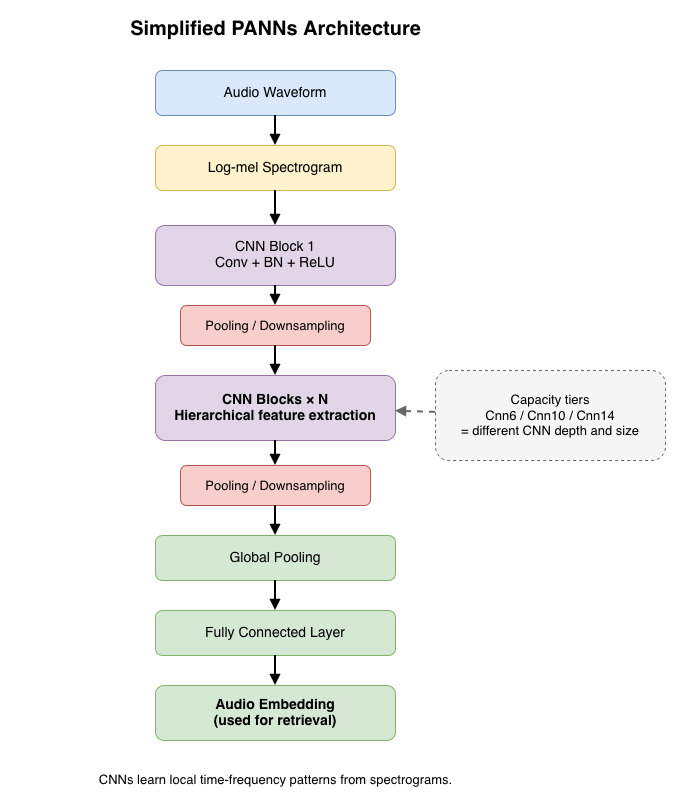
\includegraphics[width=0.55\textwidth, keepaspectratio]{diagram/archtecture/PANN-diagram.jpg}
  \caption{Simplified PANNs (CNN) architecture}
  \label{fig:pann_arch}
\end{figure}

Figure~\ref{fig:mert_arch} illustrates the MERT pre-training framework. Raw audio is first processed by a 1D convolutional feature extractor, producing a sequence of frame-level representations. These are fed into a Transformer encoder under a masked prediction objective: a subset of frames is masked, and the model learns to predict their representations as produced by two teacher networks---an acoustic teacher (based on EnCodec VQ codes) and a musical teacher (based on CQT features). This self-supervised pre-training regime on 160,000 hours of music data is what gives MERT its music-specific representations. Capacity scaling from MERT-95M to MERT-330M increases the depth and width of the Transformer encoder.

\begin{figure}[htbp]
  \centering
  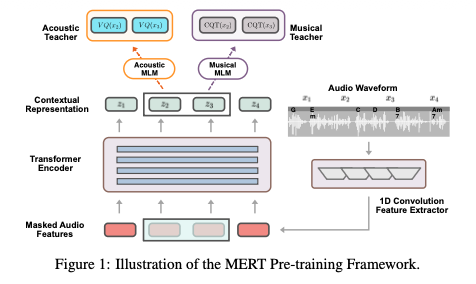
\includegraphics[width=0.75\textwidth, keepaspectratio]{diagram/archtecture/MERT-diagram.png}
  \caption{MERT pre-training framework}
  \label{fig:mert_arch}
\end{figure}

\section{Label Construction}

\textbf{Composer labels.} Composer names are normalized to a canonical form using Unicode decomposition and a hand-curated alias table, ensuring consistent matching across variant spellings and abbreviations. The normalized field is stored as a stable evaluation key, separate from the raw metadata string.

\textbf{Character labels.} Labels are derived using the arousal--valence (AV) framework \cite{eerola2011}. Each track is processed by Music2Emo \cite{music2emo2025}, a pretrained music emotion recognition model that outputs valence and arousal scores on a 1--9 scale. Scores are linearly normalized to $[0,1]$ via $\hat{x} = (x-1)/8$. Because AV predictions for classical music concentrate in a narrow mid-range region, fixed absolute thresholds are unreliable; per-dimension thresholds are set at the 33rd and 67th percentiles of the corpus distribution. This yields four binary tags:
\begin{itemize}
  \item \textit{Energetic}: arousal $\geq$ 67th percentile
  \item \textit{Calm}: arousal $\leq$ 33rd percentile
  \item \textit{Tense}: valence $\leq$ 33rd percentile
  \item \textit{Lyrical}: to capture the dense, emotionally restrained center of the classical music distribution, an inner bounding box (40th--60th percentiles on both axes) defines the neutral \textit{Lyrical} class, ensuring the most common VA profile in the dataset does not go unlabeled
\end{itemize}

These pseudo-labels are fixed prior to evaluation and reused identically across all embedding models. Because the labeling pipeline is independent of the embedding models under study, it does not introduce model-dependent labeling bias; any effect on absolute metric values is shared equally across all experimental conditions. Figure~\ref{fig:va_scatter} shows the valence--arousal distribution of the corpus and the resulting threshold boundaries.

The at-least-one-shared-label relevance criterion was chosen to maximize label coverage given the small label vocabulary (four tags). Stricter criteria, such as requiring two or more shared labels, would render many queries relevance-empty: with only four tags and a corpus of 203 tracks, requiring multi-label overlap at $K{=}5$ would produce degenerate evaluation conditions for a substantial fraction of queries. The at-least-one definition ensures that every labeled query has at least one relevant item in the corpus, preserving the validity of rank-based evaluation. A consequence is that the resulting relevance distribution is broad, which is why Recall@5 and F1@5 are structurally suppressed in the character proxy results. Stricter relevance criteria, including multi-label overlap, cosine similarity thresholds over AV scores, or expert-annotated perceptual similarity judgments, are left as directions for future work.

\begin{figure}[htbp]
  \centering
  
\includegraphics[width=0.75\textwidth, keepaspectratio]{diagram/plots/va_scatter.pdf}
  \caption{Valence--arousal scatter of the iPalpiti corpus}
  \label{fig:va_scatter}
\end{figure}

\section{Evaluation Protocol}

Each track serves as a query in a leave-one-out setting; the query item is excluded from the candidate pool. Metrics are averaged across all 203 queries. Ties are resolved using tie-aware ranking with averaged ranks. Primary evaluation relies on NDCG@5 and MAP@5 as rank-aware metrics; Hit@5 is reported as a complementary top-$K$ success indicator. Recall@5 and F1@5 are reported but interpreted with caution given the broad relevance distribution of the character proxy \cite{canamares2020, urbano2013}.

All metrics are evaluated at a cutoff of $K{=}5$, which focuses assessment on the top portion of the ranked list rather than the full ranking. This cutoff reflects the role of the embedding model as a candidate generation component: in practice, a short candidate list (typically 5--20 items) is passed to a downstream re-ranking or user-facing stage, so retrieval quality beyond the top-$K$ is operationally irrelevant at this stage. With a catalog of 203 tracks, $K{=}5$ represents approximately 2.5\% of the catalog, consistent with the selectivity expected of a candidate generation step. Smaller cutoffs ($K{=}1$, $K{=}3$) would be overly sensitive to tie-breaking; larger cutoffs ($K{=}10$, $K{=}20$) would begin to include a substantial fraction of the catalog, reducing the discrimination between models.

NDCG@$K$ is chosen as the primary ranking metric despite this study using binary relevance labels. Although NDCG is typically motivated by graded relevance, it retains a meaningful advantage over set-based metrics even in the binary case: it penalizes relevant items appearing lower in the ranking, whereas Recall@$K$ and F1@$K$ are position-insensitive and treat any ordering of the top-$K$ identically. MAP@$K$ was considered as an alternative; in binary relevance settings MAP@$K$ and NDCG@$K$ behave similarly, but NDCG@$K$ is more commonly reported in music retrieval literature \cite{urbano2013, tamm2024} and facilitates direct comparison with prior work.

Hit@$K$ is included alongside NDCG@$K$ as a complementary signal rather than a substitute. Unlike NDCG@$K$, Hit@$K$ is a binary indicator of whether \emph{any} relevant item appears in the top-$K$, independent of its rank position and independent of the size of the relevant set $|R|$. This makes Hit@$K$ robust to the dense-relevance suppression that affects Recall@$K$ and F1@$K$ when $|R|$ is large relative to $K$: it asks only whether the retrieval system surfaces at least one relevant item, which is a meaningful lower-bound signal for candidate generation. It is not used to distinguish fine-grained ranking differences between models (NDCG@$K$ serves that role), but rather to confirm that retrieval does not fail entirely for a given query.

We use standard definitions of NDCG@$K$, MAP@$K$, Hit@$K$, Recall@$K$, and F1@$K$. For query $q$, relevance is binary, $\mathrm{rel}_q(i) \in \{0,1\}$, and all metrics are computed over the top-$K$ ranked list and averaged across queries.

Five metrics are used in this evaluation. NDCG@$K$ (Normalized Discounted Cumulative Gain) is a rank-aware metric that rewards relevant items appearing higher in the list via logarithmic position discounting, normalized against the ideal ranking. MAP@$K$ (Mean Average Precision) averages precision at each rank position where a relevant item is found, rewarding both early retrieval and overall coverage within the top-$K$. Hit@$K$ is a binary signal indicating whether at least one relevant item appears in the top-$K$, independent of rank position or the size of the relevant set. Recall@$K$ measures the fraction of all relevant items in the corpus that are recovered in the top-$K$. F1@$K$ is the harmonic mean of Precision@$K$ and Recall@$K$. All metrics are averaged across all 203 queries to produce corpus-level scores.

% -----------------------------------------------
% Chapter 4: Results
% -----------------------------------------------
\chapter{Results}\label{sec:results}

\section{Sanity Proxy: Composer Retrieval}

The Sanity Proxy evaluates composer-identity retrieval, a structured task where relevance is determined by exact categorical match. Results are shown in Table~\ref{tab:sanity_results}.

\begin{table}[!htbp]
\centering
\caption{Sanity Proxy Results (Composer Retrieval)}
\label{tab:sanity_results}
\begin{tabular}{lccccc}
\hline
\textbf{Model} & \textbf{NDCG@5} & \textbf{MAP@5} & \textbf{Hit@5} & \textbf{Recall@5} & \textbf{F1@5} \\
\hline
\multicolumn{6}{c}{\textbf{CNN Family}} \\
\hline
CNN-Small  & 0.580 & 0.539 & 0.670 & 0.203 & 0.196 \\
CNN-Medium & 0.577 & 0.539 & 0.665 & 0.221 & 0.220 \\
CNN-Large  & 0.621 & 0.582 & 0.695 & 0.236 & 0.237 \\
\hline
\multicolumn{6}{c}{\textbf{Transformer Family}} \\
\hline
Transformer-Medium & 0.661 & 0.629 & 0.724 & 0.270 & 0.272 \\
Transformer-Large  & 0.615 & 0.575 & 0.690 & 0.240 & 0.231 \\
\hline
\end{tabular}
\end{table}

Scaling is non-monotonic within both families. In the CNN family, NDCG@5 dips from Small (0.580) to Medium (0.577) before recovering at Large (0.621); MAP@5 follows the same pattern (0.539, 0.539, 0.582). In the Transformer family, all metrics decrease from Medium (NDCG@5: 0.661, MAP@5: 0.629) to Large (0.615, 0.575), indicating that the larger model yields worse ranking quality on this structured task. The agreement between NDCG@5 and MAP@5 confirms the non-monotonic finding is not an artifact of metric choice. Capacity does not consistently improve composer retrieval within either family.

\section{Primary Musical Proxy: Character Retrieval}

The Musical Proxy evaluates abstract semantic retrieval based on shared affective character labels, where many items share at least one label with any given query. Results are shown in Table~\ref{tab:musical_results}.

\begin{table}[!htbp]
\centering
\caption{Primary Musical Proxy Results (Character Retrieval)}
\label{tab:musical_results}
\begin{tabular}{lccccc}
\hline
\textbf{Model} & \textbf{NDCG@5} & \textbf{MAP@5} & \textbf{Hit@5} & \textbf{Recall@5} & \textbf{F1@5} \\
\hline
\multicolumn{6}{c}{\textbf{CNN Family}} \\
\hline
CNN-Small  & 0.659 & 0.631 & 0.783 & 0.039 & 0.072 \\
CNN-Medium & 0.660 & 0.634 & 0.768 & 0.038 & 0.071 \\
CNN-Large  & 0.647 & 0.619 & 0.749 & 0.038 & 0.070 \\
\hline
\multicolumn{6}{c}{\textbf{Transformer Family}} \\
\hline
Transformer-Medium & 0.640 & 0.592 & 0.778 & 0.033 & 0.061 \\
Transformer-Large  & 0.643 & 0.597 & 0.768 & 0.036 & 0.067 \\
\hline
\end{tabular}
\end{table}

Capacity has negligible effect on character retrieval. Within the CNN family, NDCG@5 moves from 0.659 (Small) to 0.660 (Medium) to 0.647 (Large), a non-monotonic pattern with absolute differences under 0.015; MAP@5 mirrors this (0.631, 0.634, 0.619). Within the Transformer family, Medium and Large yield nearly identical scores across both rank-aware metrics (NDCG@5: 0.640 vs.\ 0.643; MAP@5: 0.592 vs.\ 0.597). Hit@5 is high across all models ($\geq$0.749), yet Recall@5 is uniformly low ($\leq$0.039) because the number of relevant items per query is large relative to the cutoff $K{=}5$: rank-aware metrics (NDCG@5, MAP@5) and the top-$K$ success indicator (Hit@5) appear to provide more informative signals in this setting than set-based metrics (Recall@5, F1@5).

\section{Embedding Extraction Cost}

Latency is measured as the average processing time per track during offline embedding extraction on an Apple Mac Mini M1 (2020), 16\,GB RAM, CPU-only, batch size 1. Table~\ref{tab:latency_results} reports extraction latency, parameter count, and embedding dimensionality for each model.

\begin{table}[!htbp]
\centering
\caption{Embedding extraction cost and model size}
\label{tab:latency_results}
\begin{tabular}{lccc}
\hline
\textbf{Model} & \textbf{Params (M)} & \textbf{Emb.\ Dim} & \textbf{Latency (ms/track)} \\
\hline
CNN-Small (Cnn6)   & 4.8  & 512  & 2178.87   \\
CNN-Medium (Cnn10) & 5.2  & 512  & 3108.93   \\
CNN-Large (Cnn14)  & 80.8 & 2048 & 4217.94   \\
Transformer-Medium & 95   & 768  & 23145.73  \\
Transformer-Large  & 330  & 1024 & 55724.24  \\
\hline
\end{tabular}
\end{table}

Embedding extraction latency increases substantially and disproportionately with model capacity across both families. Within the CNN family, latency rises from 2{,}179\,ms (Cnn6, 4.8\,M parameters) to 4{,}218\,ms (Cnn14, 80.8\,M), a ${\sim}2{\times}$ latency increase for a $17{\times}$ growth in parameter count. The disproportion is more extreme for Transformers: latency grows from 23{,}146\,ms (MERT-95M) to 55{,}724\,ms (MERT-330M), a $2.4{\times}$ increase for a $3.5{\times}$ parameter increase. Transformer-Large is ${\sim}13{\times}$ slower than CNN-Large with no corresponding ranking advantage on either task. These costs apply to offline catalog ingestion; online query time is determined by similarity search over precomputed embeddings and is independent of model size. However, ingestion cost is operationally relevant for archival systems that re-index on catalog updates or lack GPU infrastructure. Figure~\ref{fig:cost_quality} plots NDCG@5 against extraction latency for all five models on both tasks.

\begin{figure}[htbp]
  \centering
  
\includegraphics[width=\textwidth, keepaspectratio]{diagram/plots/cost_quality_scatter.pdf}
  \caption{Cost--quality trade-off across embedding models}
  \label{fig:cost_quality}
\end{figure}

\section{Summary of Empirical Findings}

The results yield three implications for candidate generation in data-constrained settings. First, capacity scaling is non-monotonic within both architectural families: larger models do not consistently outperform smaller ones, and in the Transformer family, the larger model underperforms the smaller on structured retrieval. Second, the effect of capacity is task-dependent: structured composer retrieval shows measurable variation across capacity tiers, whereas abstract character retrieval is almost entirely insensitive to model size. Third, the cost--quality ratio degrades sharply at high capacity: the largest Transformer imposes a ${\sim}25{\times}$ latency penalty relative to CNN-Small while failing to improve ranking quality on either task. For content-based candidate generation under these conditions, mid-sized models achieve comparable ranking quality at substantially lower ingestion cost.

% -----------------------------------------------
% Chapter 5: Discussion
% -----------------------------------------------
\chapter{Discussion}

\section{Capacity Scaling Does Not Justify Its Cost in This Setting}

The results indicate that increasing embedding-model capacity does not produce consistent improvements in candidate ranking quality. The effect is task-dependent: on structured composer retrieval, capacity differences produce measurable but non-monotonic variation in NDCG@5 and MAP@5; on abstract character retrieval, capacity has negligible effect across all metrics. This is consistent with prior findings that strong MIR benchmark performance does not necessarily transfer to improved retrieval quality in recommendation pipelines \cite{tamm2024}. The stylistic homogeneity of a single-domain classical archive may further compress the embedding space, reducing the discriminative advantage that additional capacity can provide.

The cost side of this trade-off is empirically clear: latency increases from 2{,}179\,ms per track (CNN-Small) to 55{,}724\,ms (Transformer-Large), a ${\sim}25{\times}$ increase, while consistent ranking gains are not observed in this setting. NDCG@5 on the structured task moves from 0.580 to 0.621 within the CNN family and peaks at 0.661 for Transformer-Medium before declining to 0.615 for Transformer-Large. The largest model in each family does not achieve the best ranking quality on either task. The return on investment from capacity scaling, measured as ranking gain per unit of ingestion cost, does not justify the overhead in this setting.

\section{System-Level Implications for Candidate Generation}

Isolating the candidate generation stage makes model selection a direct system design decision. The embedding model is the only ranking mechanism; its cost is paid at catalog ingestion with no collaborative signal to compensate, and no downstream re-ranking can recover from poor candidate quality. In this regime, the choice of embedding model has concrete operational consequences.

The results suggest that mid-sized models offer the most favorable cost--quality profile for catalog ingestion under these conditions. CNN-Small and CNN-Medium achieve NDCG@5 within 0.04 of Transformer-Medium on the structured task at ${\sim}10{\times}$ lower latency. For systems that must re-index periodically or operate without GPU infrastructure, this difference is operationally significant. Transformer-Large, by contrast, incurs the highest ingestion cost while delivering worse structured-task ranking than Transformer-Medium and no meaningful improvement on character retrieval.

These findings also indicate that the relevance structure of the retrieval task can have a stronger effect than model size on metric behavior in this setting. When relevant items are broadly distributed, as in the character proxy, Recall@5 and F1@5 remain low regardless of model, while NDCG@5 and MAP@5 remain stable and Hit@5 remains high. Practitioners designing offline evaluation protocols for cold-start candidate generation may benefit from aligning metric choice with the expected relevance distribution of their catalog.

\section{Limitations}

This study has four primary limitations. First, while the dataset scale ($N{=}203$) is intentionally small, it serves as a high-density, controlled stress-test for embedding space geometry: if massive capacity scaling fails to resolve semantic overlap in this curated environment, it is highly unlikely to justify its computational overhead in larger, heterogeneous catalogs. Second, to isolate the candidate generation stage, we evaluate pure item-to-item similarity without modeling downstream user-level personalization or re-ranking. Third, while character pseudo-labels were manually validated for consistency, their initial generation via pretrained models may introduce systemic biases; because these labels are fixed across all evaluated embeddings, however, they affect absolute metric values rather than the relative capacity comparisons that form our core findings. Finally, mean-pooling of segment-level embeddings may dilute localized semantic variations within long-form classical recordings, potentially limiting the ability of high-capacity models to exploit fine-grained temporal structure; future work should explore sequence-aware aggregation methods to better preserve such information.

\section{Directions for Future Work}

An immediate next step is to evaluate whether the observed cost--quality trade-off persists in larger, heterogeneous catalogs, where increased variability may alter the marginal utility of capacity scaling. Richer semantic labels, including expert annotations or listener-derived similarity judgments, would improve the sensitivity of the abstract retrieval task and reduce reliance on pseudo-labels. Connecting the candidate generation stage to downstream re-ranking and user modeling components would establish whether the ranking differences observed here have measurable impact on end-to-end recommendation quality.

A complementary direction is to incorporate additional editorial metadata, such as instrument configuration, historical period, or ensemble size, into the retrieval pipeline alongside audio embeddings. The iPalpiti archive contains rich structured metadata of this kind, and hybrid retrieval signals that combine embedding-based similarity with metadata filtering could improve candidate quality without increasing embedding extraction cost. The present study deliberately isolates the audio embedding contribution in order to establish a clean baseline; understanding how metadata and audio signals interact in cold-start candidate generation is a natural and tractable next step that does not require user interaction data.

Once sufficient user interaction data becomes available, qualitative case studies would strengthen the empirical picture: presenting the top-5 retrieved tracks for representative queries side by side across model capacity tiers would concretely illustrate what non-monotonic scaling looks like at the item level, and whether ranking differences that appear small in aggregate metrics translate into meaningfully different candidate lists in practice.

% -----------------------------------------------
% Chapter 6: Conclusion
% -----------------------------------------------
\chapter{Conclusion}

We evaluated the effect of embedding-model capacity on candidate ranking quality for cold-start content-based music retrieval, using CNN-based and Transformer-based pretrained audio models across discrete capacity tiers. Capacity scaling is non-monotonic within both architectural families and task-dependent across them: structured composer retrieval shows measurable but inconsistent variation with capacity, while abstract character retrieval is largely insensitive to model size. In neither case do we observe consistent ranking gains from the largest model.

The cost side of this trade-off is empirically clear. Embedding extraction latency grows from 2{,}179\,ms per track (CNN-Small) to 55{,}724\,ms (Transformer-Large), a ${\sim}25{\times}$ increase, without a corresponding improvement in NDCG@5 or MAP@5. When relevant items are broadly distributed relative to the evaluation cutoff, set-based metrics such as Recall@5 and F1@5 can be suppressed regardless of ranking quality; rank-aware metrics appear to provide more reliable signals in this setting.

For practitioners building content-based candidate generation pipelines under cold-start and resource-constrained conditions, these results indicate that mid-sized models offer the most favorable cost--quality profile. Defaulting to larger models is not justified by the evidence in this setting: the ingestion overhead is substantial, while ranking gains remain inconsistent. Code and evaluation scripts are publicly available at: \url{https://github.com/cpp-iPalpiti-pilot/iPalpiti-recsys-pipeline}.

% -----------------------------------------------
% References (Step 9: continue Arabic page numbers)
% -----------------------------------------------
\SuppChap
\bibliographystyle{IEEEtran}
\bibliography{biblio}

\end{document}
